\chapter{Discussion and perspectives} % Main chapter title
\addcontentsline{toc}{chapter}{Discussion and perspectives}  
\pagestyle{plain} % remove headers/footers from the chapter page
\startcontents[chapters]

By the end of this thesis, we have developed next-generation foundation models for single-cell data and established new methodologies for their evaluation and application. This work began with the goal of improving \gls{GRN} inference from \gls{scRNA-seq} data while understanding how single-cell foundation models work. Through three chapters, we systematically addressed fundamental challenges in the field, from architectural design to cross-scale learning and rigorous benchmarking.

\textbf{scPRINT: Establishing foundations for gene network inference.} In our first chapter, we demonstrated that transformer-based foundation models pretrained on large-scale single-cell data can extract meaningful gene regulatory networks without requiring graph-structured inputs. Training on 50 million cells, we showed that several key innovations were critical: protein-based gene encodings using \gls{ESM}2 embeddings enabled cross-species generalization while reducing parameters; learned expression tokenization via \gls{MLP}s outperformed hand-crafted binning; and genomic positional encodings captured co-regulation patterns. We learned that the transformer's attention matrices, when properly extracted and filtered through head selection mechanisms, could recover cell-type-specific regulatory interactions that outperformed traditional methods like GENIE3 on the Omnipath benchmark. \cite{badia-i-mompelGeneRegulatoryNetwork2023}

Perhaps most importantly, we learned that the lack of standardized evaluation was hindering progress in the field. Our creation of BenGRN and GRnnData addressed this gap, enabling fair comparisons across methods using multiple ground truth types, from literature-based networks to cell-type-specific \gls{ChIP-seq}/perturb-seq intersections and genome-wide perturb-seq data. \cite{dixitPerturbseqDissectingMolecular2016} We showed that \gls{scPRINT} not only excelled at network inference but also achieved competitive zero-shot performance on orthogonal tasks like cell type annotation, batch correction, and denoising, demonstrating that these capabilities emerge naturally from learning good cellular representations. The application to prostate tissue revealed early \gls{TME} markers in rare B-cells and differential hub genes in \gls{BPH}-associated fibroblasts, validating the model's utility for biological discovery. This chapter led to a publication in Nature Communications.

\textbf{Xpressor: Learning across biological scales.} Our second chapter addressed a fundamental limitation: foundation models at different biological scales (molecules, sequences, cells, tissues) operated in isolation, unable to leverage information flow between scales. We learned that cross-attention-based compression mechanisms could effectively transform high-dimensional gene-level representations into lower-dimensional cell-state vectors while preserving biological information. The Xpressor architecture, grounded in information bottleneck theory \cite{chechikInformationBottleneckGaussian}, demonstrated that explicit compression and decompression through learned latent tokens outperformed simple pooling strategies, improving cell-type prediction and embedding quality.

More significantly, we showed that lower-scale models could be enriched through adapter-based fine-tuning on upper-scale tasks. By adding trainable \gls{MLP} adapters to \gls{ESM}2 protein embeddings during \gls{scPRINT} pretraining, we demonstrated that protein sequence representations could be augmented with co-expression information learned from millions of single-cell profiles. This multi-scale fine-tuning improved cell-type prediction by and gene network inference compared to frozen embeddings, proving that information truly flows bidirectionally between scales. We learned that each biological scale's vocabulary can be viewed as compressed representations of the scale below, and that explicit architectural support for this compression---rather than ad-hoc concatenation---is essential for effective cross-scale learning. This chapter led to a poster at ICML 2025 F4MLS workshop and is currently under a second review for publication in Bioinformatics Advances.

\textbf{scPRINT-2: Systematic validation and next-generation capabilities.} In our third chapter, we addressed the field's critical gap in understanding which design decisions matter most. Through an unprecedented additive benchmarking framework evaluating 42 model variants across multiple seeds, we systematically quantified the impact of each architectural choice. We learned that denoising outperforms masking as a pretraining task; un-normalized expression is superior to normalized input; \gls{ESM}-based gene tokens significantly outperform learned embeddings; genomic location encoding accelerates convergence; and model size correlates strongly with performance on complex tasks like network inference.

Training on 350 million cells from 16 organisms---the largest single-cell corpus assembled to date---we learned that data diversity and quality matter more than sheer quantity. Reducing to 200 human datasets caused minimal performance loss, while using low-diversity datasets alone caused performance to plummet. We showed that cluster-weighted and \gls{NNZ}-weighted sampling strategies were essential for training effectively on such heterogeneous data. The incorporation of 12 validated innovations, including the XPressor architecture, \gls{GNN}-based expression encoders, and criss-cross attention, resulted in state-of-the-art performance in zero-shot cell-type classification on Open Problems (surpassing all existing methods), superior expression denoising across all contexts, and best-in-class batch integration.

Critically, we demonstrated that \gls{scPRINT}-2 generalizes beyond its training distribution. On Xenium spatial transcriptomics (an unseen modality), it successfully denoised expression, imputed 5,000 unseen genes, and produced meaningful predictions. On cat and tiger tissues (unseen organisms), it achieved enough accuracy across 500 cell types to sometime correct expert annotations. The XPressor architecture enabled counterfactual generation, allowing us to ``humanize'' mouse expression profiles with strong enrichment in correctly predicted differentially expressed genes. We learned that meaningful gene embeddings---enriched for biological pathways rather than mere expression values---emerge only with proper architectural support for compression and reconstruction. This chapter led to a preprint, currently under review in Nature Methods.

\textbf{Key learnings and paradigm shifts.} Across these three chapters, several overarching insights emerged. First, we learned that \gls{GNN}s, despite initial promise, were not the optimal approach for single-cell data due to the absence of known graph structures and poor scaling properties. Transformers, which can be viewed as \gls{GNN}s on fully-connected graphs, proved superior when architectural innovations addressed their quadratic complexity. Second, we learned that foundation model evaluation in genomics had been inadequate, relying on artificial benchmarks disconnected from biological reality and real-world applicability. Our systematic benchmarking revealed that many claimed capabilities of existing models were overstated or poorly validated. Third, we learned that accessibility and reproducibility are as important as model performance---releasing not just weights but also training code, datasets, tutorials, and documentation was essential for community adoption and scientific progress.

But a lot of work remains at the crossroads of AI and biology. In the following sections, I will discuss some of the challenges and opportunities that I see in this space.

\section{Collecting data in the wild}

\subsection{Genetic diversity}

The first issue to address for a better model will be obtaining cell expression data across a much more diverse genetic background. This also means sequencing the genome of the tissues we are analyzing, which is rarely done because genomic data has strong laws surrounding patient anonymity and public sharing.

Fortunately, we have seen projects starting around this goal, such as the 10K10K, which aims to sequence 10,000 cells from 10,000 people along with genetic data \cite{cuomoImpactRareCommon2025}. The Sanger Institute is also doing something similar with spatial transcriptomics of 10,000s of samples in development, along with their genomes.

\begin{figure}[ht]
  \centering
  \includegraphics[width=0.9\textwidth]{./figures/popvar.png}
  \caption{the genetic diversity in single cell dataset highlited with mr.vi. \cite{boyeauDeepGenerativeModeling2025a}}
  \label{fig:genediv}
\end{figure}

But these remain small-scale projects compared to the diversity of life on Earth. In genomics, scBasecamp \cite{youngblutScBaseCount2025} and other for-profit companies are working on sampling life around the world from barren places to ocean depths, with the stated goal of developing higher quality models. Single-cell models would stand to benefit just as much.

\subsection{Interventional data}

Finally, we also want interventional datasets. Currently, perturb-seq datasets with tens of thousands of perturbations exist, such as the genome-wide perturb-seq dataset and Tahoe-100M \cite{zhangTahoe100M2025}. However, here too, the scale remains too small. The Broad \& Sanger Institute's PRISM \cite{arafehPresentFutureCancer2025} and DepMap projects examined millions of perturbations, albeit without deep phenotypic readouts. Recursion \cite{fayRxRx3PhenomicsMap2023} assessed image-based perturbations across at least as many, while Xaira \cite{huangXAtlasOrionGenomewide2025} has started to release a dual gene knockout dataset of unparalleled quality.

\subsection{Data quality}

Indeed, the second missing important axis is data quality. Genomics is plagued with very low-quality, noisy, or biased, poorly labeled datasets. This is due to the high cost of sequencing, the complex chemistry of the experiments, and the poor academic incentives driving the creation of these datasets.

It leads to an unstate Pareto front, where we want both more depth and more breadth: more diversity versus more quality.

\begin{figure}[ht]
  \centering
  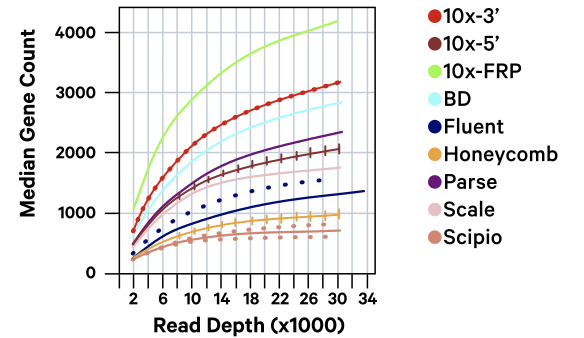
\includegraphics[width=0.9\textwidth]{./figures/sequal.png}
  \caption{The number of genes detected per reads for different single-cell technologies.}
  \label{fig:sequal}
\end{figure}

It might be solved by new technologies, indeed we now have technologies like VASA-seq \cite{salmenHighthroughputTotalRNA2022}, 10X's Flex \cite{llora-batlle10xGenomicsGene2024}, and smart-seq 3 \cite{hagemann-jensenSinglecellRNACounting2020} that promise unparalleled definition for a given sequencing budget. The number of genes they can discover per cell, which is a measure of quality of the sequencing has increased by 50\% compared to 10x v3. 

Another issue is the set of cells that can be assessed and their fidelity to what was initially sent for sequencing. 10x's Xenium, BGI's STEREO-seq, and expansion-based in situ method~ \cite{alonExpansionSequencingSpatially2021} are promising for sequencing RNAs in their original 2D or even 3D context within sub-cellular locations for millions of cells at once. Without manupulating the cells and creating droplets. Solving many issues of current technologies. But we will also have to be smarter in how we select cells to sequence. 

\section{Multi modality \& perturbations}

Indeed, these two modalities and their tradeoffs exist within a range of other techniques often needed to make sense of RNA biology itself.

Interventional data is also required for the model to learn causality, especially when assessed at multiple fine-grained timescales and in higher-quality cellular models such as organoids. Imaging-based methods can also achieve higher throughput, lower prices without destroying the cells.

\begin{figure}[ht]
  \centering
  \includegraphics[width=0.9\textwidth]{./figures/minibrains.png}
  \caption{Image of brain organoids from the Broad Institute}
  \label{fig:organoids}
\end{figure}

But the search space remains unfathomable. it is not just every genes that one would want to perturb, it is the hundreds of millions of locations that might create a specific effect. It is not just in one cell but in the many possible cell states. It is not just one element but multiple at a time, not just one time point but many, not just one readout. Tools like digital microfluidics \cite{yuFieldProgrammableDigital2023} might allow us to solve some of these problems by providing precise control over which cells receive specific perturbations and obtain particular readouts, instead of pooling experiments and sequencing budgets randomly. If paired with AI models and online active learning, we might some day, have a shot at creating a true AI-virtual cell.

\section{The AI virtual cell}

We have seen barely glimpses of the idea of an AI-based virtual cell modeling in this thesis. But it is undeniably through the above-mentioned techniques that more work will be needed. Indeed, the goal of an virtual cell is to be able to predict the state of a cell through time, as it interacts with and gets perturbed by its environment. With the advent of \gls{CRISPR}-screens, and drug-seq, a focus has been put on predicting the effect of a drug on a dissociated cell after a given period of time. this can be on: its survival, its morphology or its expression profile. Many big projects have been launched such as DepMap \cite{DepMapPanCancerBiomarker} and Recursion's RxRx database \cite{fayRxRx3PhenomicsMap2023}. More recently, the Arc Virtual Cell Challenge \cite{bunneHowBuildVirtual2024}, also highlighted how limited our current technology and benchmarks are, with AI models achieving poor performances, the limited usability of cross-lab data and metrics that were easily gamed.

But most data is and will remain generated through the thousands of labs across the world. Most of the time siloed. Training on these public noisy, static and poorly labelled datasets is often called pretraining. While the above-mentionned techniques could be seen as reinforcement learning with active feedback (RLAF). Such an AI-VC model would have been pretrained on most of the available biological data, using foundation models of single-cell multimodalities, tissues, molecules, and protein-RNA-DNA sequences, pooled together in the kind of approaches we described in Chapter 2. LLMs could allow rich reasoning across these representations, results, and the breadth of written human knowledge.

Finally, the hope is to drive experiments in the lab and perform hypothesis generations that could be transfered from cheap in silico experiments to more expensive in vitro experiments on dissociated cells, organoids and finally to in vivo models. This loop of pretraining, RLAF, and hypothesis generation is what we call the lab in the loop approach to cellular modeling (Figure \ref{fig:labinloop}).

\begin{figure}[ht]
  \centering
  \includegraphics[width=0.9\textwidth]{./figures/lab-in-the-loop.jpg}
  \caption{overview of the lab in the loop approach to cellular modeling. from the AIVC perspective paper \cite{bunneHowBuildVirtual2024}.}
  \label{fig:labinloop}
\end{figure}

Many challenges remain in bridging fields such as data engineering, machine learning, material engineering, microelectronics, molecular biology, and cell biology, but the rewards are tremendous, as many diseases won't be solved by brute force approach or by targeting one specific gene, whether cancer or other complex multi-cellular aging diseases.

\newpage\thispagestyle{empty}